\section{Protocol-Fixed Mission2 Follow-up}
\label{sec:mission2}
\subsection{Selection and the execution record}
Mission2 source integrity and six-channel synchronization are audited without
resampling, filling, or intersecting away observations. Original values are
losslessly representable by the binary32 schema. Channel selection uses metadata
rather than anomaly scores: channels 86--91 are the lowest numbered complete group
of six numeric target channels. The study and implementation are committed as
\texttt{3c1ed90} before annotation conversion. The complete input/code/environment
lock is committed as \texttt{d5366f3} before evaluation. Runtime checks reject
uncommitted or changed study code; temporal and primary analyses verify the same
record. This is a local Git execution record, not third-party preregistration or
proof that labels were never viewed.

The follow-up includes 3,675,510 evaluation observations and 15,312 active hours.
Receivers use 3,698,356 eligible training observations; AR(1) uses 3,698,338 eligible
pairs. Retention settings remain unchanged. Four capture conditions, four recording
controls including pairs, uniform, and ten-seed reservoir/random-phase controls
give 148 capture arms. Nine selected policies at four caps give 36 temporal
assessments. Every declared arm completes, and the primary contrast is analyzed
without changing the group, split, cap, or seeds.

\subsection{The primary comparison is uninformative}
The fixed source channels contain 252 annotation rows, all classified as rare
nominal events. The evaluation interval includes 150 such rows across 25 event IDs
and \emph{no anomaly annotations}. An independent raw-CSV category/interval check
agrees with the prepared bundle. The empty eligible anomaly set is therefore not
a decoding failure, a policy losing every event, or all anomalies being censored.

Under the frozen exclusion rules, rare events cannot be relabeled as faults to
supply a denominator. Eligible and full-archive-recoverable anomaly counts are
both zero; the primary paired outcome table is empty. Event recall and an effect
estimate are unavailable, not zero or perfect. The primary result is explicitly
\emph{uninformative}. No alternate group is substituted after observing this.
This attempt supplies no confirmation or refutation of Mission1 fault-recovery
performance, despite completing the software and transfer workflow.

\subsection{Secondary temporal input availability}
At the 1,024-byte cap, paired background retains 45,935 scorable original transitions
versus zero for singleton background. The complete evaluation source has 3,675,508
adjacent pairs within the gap limit, so the paired control makes 1.25\% available.
The encoded streams differ by 36 bytes: 3,797,304 for pairs and 3,797,268 for
singletons, both rounding to 3.62 MiB. The first-difference threshold-only stream contains headers but no raw records
on this evaluation subset, so its enabled adaptive recorder also relies on
background sampling. These counts concern captured inputs before
delivery and include intervals excluded from fault scoring. They validate the
structural availability tradeoff on another source; they do not measure anomaly
recall or physical diagnostic benefit.

\begin{table}[htbp]
\centering\small
% Generated from the completed frozen Mission2 reports; N/A is not zero recall.
\begin{tabular}{lrrrr}
\toprule
Capture / policy & MiB & PCA events & AR(1) events & Scorable pairs \\
\midrule
Uniform & 14.66 & N/A & N/A & 0 \\
Difference / adaptive & 3.62 & N/A & N/A & 0 \\
Difference / coverage & 3.62 & N/A & N/A & 783 \\
Difference / pairs & 3.62 & N/A & N/A & 45,935 \\
Disabled / singleton & 3.62 & N/A & N/A & 0 \\
Disabled / pairs & 3.62 & N/A & N/A & 45,935 \\
\bottomrule
\end{tabular}

\caption{Mission2 at 1,024 bytes per active hour. N/A marks unavailable event
metrics because the fixed evaluation subset has no eligible anomalies. Consecutive
input availability and actual byte cost remain measurable.}
\label{tab:mission2}
\end{table}

This is an input/task qualification limitation in our study, not an error in
the released annotations. The follow-up shows that a metadata target flag
does not guarantee anomaly-label support under the anomaly-only scoring rules for the selected representation and split.
A subsequent study should declare an annotation-only support check or evaluate the
complete intended target set before interpreting fault-retention performance. The
six-channel codec should not silently dictate a convenient subset, and the present
empty-denominator attempt must remain in the record.

\begin{figure}[htbp]
\centering
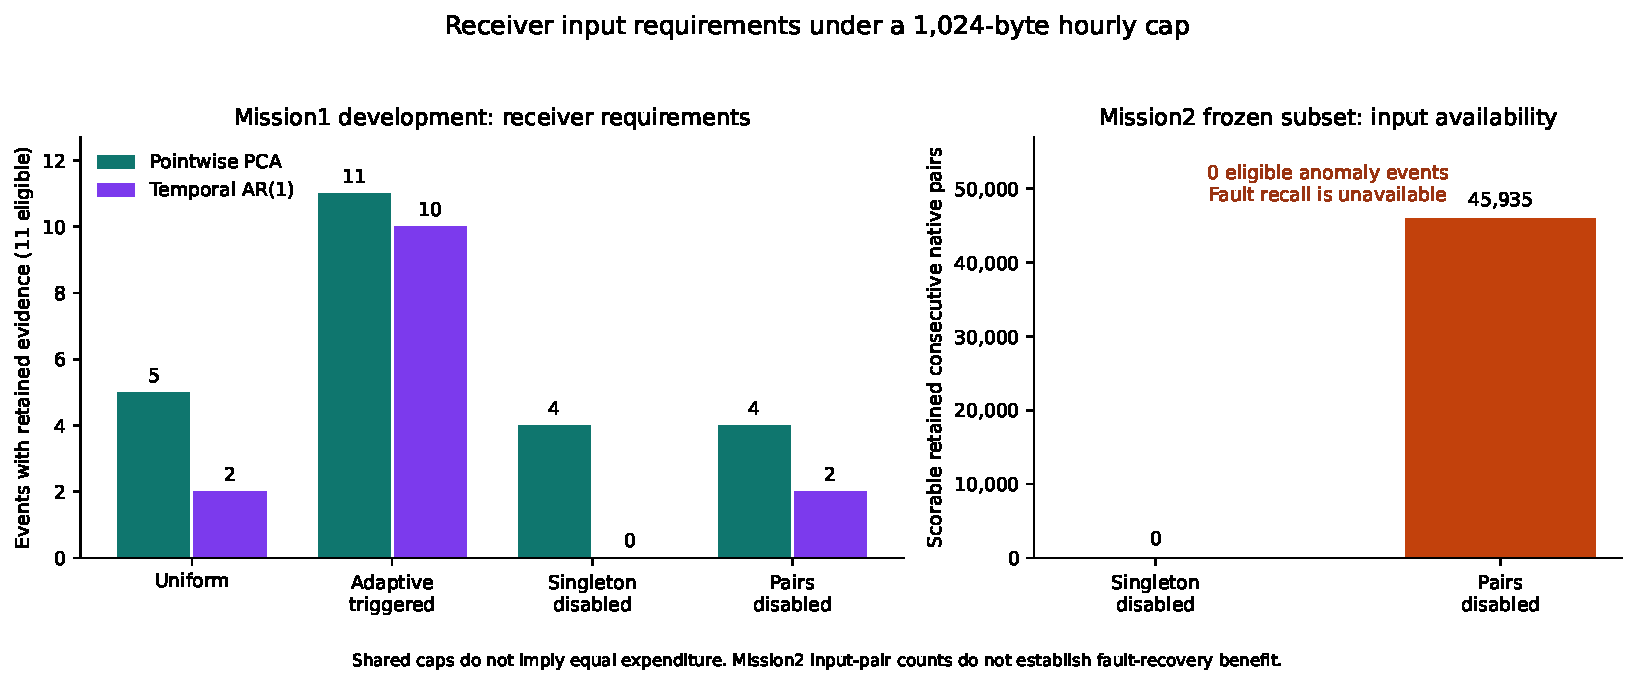
\includegraphics[width=\linewidth]{generated/receiver_requirements.pdf}
\caption{Different claims supported by the two phases. Left: Mission1 development
counts out of 11 eligible anomalies; the paired control is exploratory. Right:
Mission2 captured temporal inputs under the frozen settings, with no eligible
anomaly events. The right panel is not a fault-recovery comparison. Shared caps
need not imply equal expenditure.}
\label{fig:requirements}
\end{figure}
